\documentclass{article}

\usepackage{listings}
\usepackage{multicol}
\usepackage{tikz}
\usepackage{fancyhdr} % Fancy headers and footers
\usepackage{amsthm, amsmath, amsfonts, amssymb, mathrsfs, mathtools} % Math packages
\usepackage{enumitem}
\usepackage{geometry}
\usepackage{marginnote}

%% For inkspace figures:
\usepackage{import}
\usepackage{xifthen}
\usepackage{pdfpages}
\usepackage{transparent}
\newcommand{\incfig}[1]{%
    \def\svgwidth{\columnwidth}
    \import{./figures/}{#1.pdf_tex}
}
\pdfsuppresswarningpagegroup=1

\usepackage[plain]{algorithm}                                                   
\usepackage{algpseudocode}
\usepackage{caption}

\definecolor{Brown}{cmyk}{0,0.81,1,0.60}
\definecolor{OliveGreen}{cmyk}{0.64,0,0.95,0.40}
\definecolor{CadetBlue}{cmyk}{0.62,0.57,0.23,0}
\definecolor{lightlightgray}{gray}{0.9}

\lstset{
language=Python,                             % Code langugage
basicstyle=\ttdefault,                   % Code font, Examples: \footnotesize, \ttfamily
keywordstyle=\color{OliveGreen},        % Keywords font ('*' = uppercase)
commentstyle=\color{gray},              % Comments font
numbers=left,                           % Line nums position
numberstyle=\tiny,                      % Line-numbers fonts
stepnumber=1,                           % Step between two line-numbers
numbersep=5pt,                          % How far are line-numbers from code
backgroundcolor=\color{lightlightgray}, % Choose background color
frame=none,                             % A frame around the code
tabsize=2,                              % Default tab size
captionpos=b,                           % Caption-position = bottom
breaklines=true,                        % Automatic line breaking?
breakatwhitespace=false,                % Automatic breaks only at whitespace?
showspaces=false,                       % Dont make spaces visible
showtabs=false,                         % Dont make tabls visible
columns=flexible,                       % Column format
}



%% Set document margin:
\geometry{margin=1in} %% Add paperheight=16383pt to make page continuous


\newtheorem{theorem}{Theorem}[section]
\newtheorem{corollary}{Corollary}[theorem]
\newtheorem{lemma}[theorem]{Lemma}
\newtheorem*{remark}{Remark}
\theoremstyle{definition}
\newtheorem{definition}{Definition}[section]

\newtheoremstyle{note}{3pt}{3pt}{\normalfont}{}{\bfseries}{:}{ }{}
\theoremstyle{note}
\newtheorem*{note}{Note}

%% Margin Notes
\let\oldmarginpar\marginpar
\renewcommand{\marginpar}[2][text width=3cm, rectangle, draw,rounded corners, thick]{%
        \oldmarginpar{%
        \tikz \node at (0,0) [#1]{#2};}%
        }


%% Header and Footer
\pagestyle{fancy}
\fancyhf{}
\lhead{\classname} % Left Header text
\rhead{} % Right header text
\rfoot{Page \thepage}


%%% ADD OPTIONAL HEADER AND FOOTER RULES

%%% CHANGE SNIPPETS _ AND ^ TO DETECT IF
%%% {} HAVE ALREADY BEEN WRITTEN


%%% INPUTS %%%%%%%%%%%%%%%%%%%%%%%%%%%%%%%%%%%
\newcommand{\classname}{}


%%% SNIPPET COMMANDS %%%%%%%%%%%%%%%%%%%%%%%%%%%%%%%%%%%%%


%%%%%%%%%%%%%%%%%%%%%%%%%%%%%%%% Random stuff
% ital - \textit{}
% bld - \textbf{}
% margin - \marginnote{text}[offset]

%%%%%%%%%%%%%%%%%%%%%%%%%%%%%%%% Random math stuff
% dx  - \frac{\\partial $1}{\\partial $2}
% rarrow - \\rightarrow
% func - \\$1 : \\mathbb{$2} \\rightarrow \\mathbb{$3}, x \\mapsto 
% txt - \text{$1}
% // - \\frac{$1}{$2}$0
% sum -  \\sum \\limits $0
% qed - qed symbol (filled)
% inv - inverse ^{-1}
% mmath - $ input $ 

%%%%%%%%%%%%%%%%%%%%%%%%%%%%%%%% Environments
% align - \begin{alignedat}{4}
% props - \align{} - Numbered
% bm - \\begin{bmatrix} $1 \\end{bmatrix}
% pm - \\begin{pmatrix} $1 \\end{pmatrix}
% thm - \\begin{thm}{$1} $1 \end{thm}
% def - \\begin{def}{$1} $1 \end{def}
% lemma - \begin{lemma}
% cor - corollary \begin{corollary}
% proof - \begin{proof}
% remark - \begin{remark}
% dm -  \[\]
% beg - \begin{$1} \end{$1}
% python - \begin{lstlisting}[language=Python,escapeinside={(*}{*)}, basicstyle=\fontsize{11}{13}]
% section -  \section{}
% subsection -  \subsection{}

%%%%%%%%%%%%%%%%%%%%%%%%%%%%%%%% Constants
% reals - \mathbb{R}
% rationals - \mathbb{Q}
% integers - \mathbb{Z}
% complex - \mathbb{C}
% eps -  \\epsilon
% sig - \\sigma
% Sig - \\Sigma
% prime - ^{\prime}
% alpha - \\alpha
% beta - \\beta



%%%% START OF DOCUMENT ############
\begin{document}
\section*{MAML Problem formulation}

\begin{itemize}
    \item Each task is a MDP with horizon $ H $ .
    \item Each task $ \mathcal{T} _ {i} $ contains initial 
    state distribution $ q _ {i} (x _ {1}) $ and transition distribution
    $ q _ {i} (x _ {t+1} \mid x _ {t} , a _ {t}) $ 
    \item Model being learned $ f _ {\theta}: X _ {t} \rightarrow A _ {t} $,
    where $X_ {t}$ is the set of states at time $ t $  and $ A _ {t} $  is the set of actions at time $ t $.
    Such that $ t \in \{ 1, ..., H\} $ 
    \item The loss for task $ \mathcal{T} _ {i} $ and model $ f _ {\phi} $ is given by:\\
    \[
    L _ {\mathcal{T} _ {i} } ( f _ {\phi}) = 
    - \mathbb{E} _ {x_ {t}, a _ {t} \sim f _ {\phi}, q \mathcal{T}_ {i}} 
    \left [ \sum \limits _ {t=1} ^ {H} R_ {i} (x _ {t}, a_ {t})\right]
    \]
    \item Uses Policy gradient methods to estimate gradient both for model and meta-optimization, 
    because the dynamics are unknown. Also have the option of using trust region optim.
\end{itemize}


\newpage
\subsection*{VPG Pseudo Code (Spinning Up)}
https://spinningup.openai.com/en/latest/algorithms/vpg.html\\
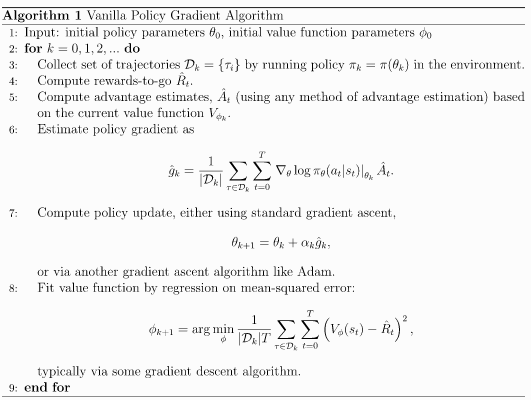
\includegraphics[scale=0.5]{./vpg.png}\\
\subsection*{TRPO Pseudo Code (Spinning Up)}
https://spinningup.openai.com/en/latest/algorithms/trpo.html\\
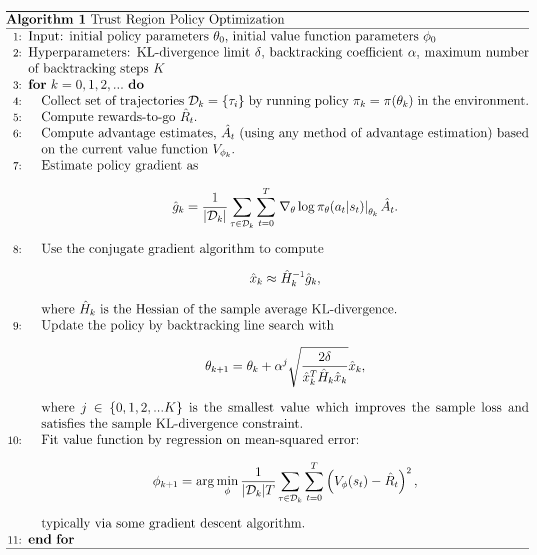
\includegraphics[scale=0.5]{./trpo.png}

%def get_model_update():
%    # Get change in each param for self.model from self.model_copy
%    diff = []
%    for each param in self.model, self.model_copy: 
%        difference = model_copy_param - model_param
%        diff.append(difference)
%    return diff

\newpage
\subsection*{Pseudo Code}
\begin{lstlisting}[language=Python,escapeinside={(*}{*)}, basicstyle=\fontsize{9}{9}\ttfamily]
def task_rollout(task):
     
    cumulative_disc_rew = 0

    for i in range(run_length):

        observation = get_observation()
        action = self.model(observation)

        disc_reward, log_prob = step(action)  # Discounted reward, log prob from action distrib
        cumulative_disc_rew += disc_reward * log_prob  ### UNSURE ABOUT THIS ##################

        if run is done: # if in terminal state, or run_length reached
            return cumulative_disc_rew  


def sample_trajectories(task, K):

    rewards_for_task = torch.zeros(K) # Cumulative sum of rewards * logprob for each K task 
    for i in range(K):
        cumulative_rew = task_rollout(task)
        rewards_for_task[i] = cumulative_rew

    return rewards_for_task  


def train_maml():
    Tasks = [t_1, t_2, t_3, ..., t_n] # List of tasks 
    K: int                             # Number of rollouts per task
    kl_div = []                       # KL divergence for each model distrib. after update
    updated_model_reward = []

    while not done:
        for task in Tasks:

            self.model = copy.deepcopy(self.meta)   # copy meta model for EACH sample 
            exp_rewards_for_tasks = sample_trajectories(task, K)
            
            ### Update self.model with VPG
            loss = - exp_rewards_for_tasks.mean() # (Eq 4 in paper, and line 6 in VPG)
            loss.backward()  
            self.optim.step()
            
            exp_rews_updated_model = sample_trajectories(task, K)
            updated_model_reward.append(exp_rews_updated_model)

            # KL Div. of updated and old policy
            kl = torch.kl_divergence(self.model._distrib, self.meta._distrib)
            kl_div.append(kl)
        
        ### Update self.meta with TRPO
        meta_grad = 0
        for exp_rew in updated_model_reward:
            meta_grad += - exp_rew.mean()  
        meta_grad.backward() # This is g_k in TRPO, line 10 in MAML code
        #  meta_grad will be same size as network self.model
        ### UNSURE HERE ^^^^^ ########################

        # KL Divergence can be computed for some non closed form sample, we can say model is actually some unknown distrib.
        kl_average = kl_div.mean(axis=1) # axis=1, i.e. (10x5) -> (10x1)
        kl_hessian = compute_hessian(kl_average) # size: ((obs_dim x obs_dim) x action_dim)???
        x = inverse(kl_hessian) * meta_grad     # Line 8 in TRPO pseudo code, exchange w/ conj. grad?
        ### UNSURE HERE ^^^^^ ########################

        update_val = backtrack_line_search(kl_hessian, x)  # Line 9 in TRPO pseudo code
        self.meta = update_model(update_val)   # Update model parameters 
self.meta = torch_network()
self.model = None
train()


### Questions ---
"""



Paper says: "In order to avoid computing third derivatives, we  use  finite  differences  to  compute  the  Hessian-vectorproducts  for  TRPO.
Where is this 3rd derivative? If I'm not mistaken it should be in the backtracking line search?

"""
\end{lstlisting}


\end{document}




